\section{Results}

%B: IMO each instance of "(Figure 2(X))" ought be replaced with "(Figure 2x)", so that (Figure 2(A)) becomes (Figure 2a). Double-parentheses should be reserved for equations and we already use caps, for example C and D, for traits. I am happy to make the change in the text, which is trivial, but I am not sure how the PDF conversion through illustrator would fare.
 
\subsection{Polyploidy and Diversification Models}
Similarly to the results obtained by \citet{mayrose_2011} and \citet{mayrose_2015}, we found that in the D/P polyploidy model the net diversification of diploids is larger than the the net diversification of polyploids since the net diversification distributions do not overlap (Figure 2(A)). This result holds true whether or not the diploidization parameter is present. However, in the presence of  the diploidization parameter the net diversification rate of polyploids is nonnegative with probability 1 (Figure 2(A)), whereas in the absence of diploidization the net diversification rate of polyploids can be negative with a probability 0.87 (FIGURE 3(A)). In terms of the relative extinction, when the diploidization parameter is present both polyploids and diploids have posterior distributions that overlap, but that pattern changes in the absence of the diploidization parameter leading to a significant difference between relative extinction where polyploids have a significant higher relative extinction rate (see Supplementary Information).\newline

For the D/P+A/B model with diploididization the diploid and polyploid net diversification rates are overlapping for both state A and B of the hidden trait (Figure 2(B)). In this model, the differences in net diversification are due to the presence of a hidden trait and not to the differences in ploidy. When diploidization parameter is absent the hidden state is still driving the differences in diversification rates (Figure 3(B)).

\subsection{Polyploidy and Breeding System models}
When breeding system is considered simultaneously from polyploidy, we found that in the ID/CD/CP model self-incompatible and diploid state (ID) has significantly larger net diversification rate compare to both self-compatible diploid (SD) and polyploid rates(CP). Meanwhile, both self-compatible diploid and polyploid net diversification rates have overlapping posterior distributions (Figure 2(E)). When hidden state was added, the ID/P/CD+A/B model, significant differences between self-compatible and self-incompatible diploids continue to be the truth for both A and B values of the hidden state. However, the posterior distribution for the net diversification rate of polyploids overlaps with both the self-compatible and self-incompatible posterior distributions for each value of the hidden state (Figure 2F). This result indicated that polyploid state was not significantly different from diploid from the net diversification perspective.  In the absence of diploidization, models ID/CD/CP no $/delta$ and ID/P/CD no $delta$ +A/B showed that the net diversification of polyploids is equivalent to the net diversification of self-compatible diploids. In the absence of diploidization, the net diversification rates of self-incompatible diploids are always faster than their self-compatible diploid and polyploid counterparts (Figures 3C and 3D). \newline
Polyploidization rates from self-compatible diploid $\rho_{CD}$ and from self-incompatible diploid $\rho_{ID}$ are not significantly different (see supplementary information figures). However, the distribution of $\rho_{ID}$ seems to always consider faster values compare to the distribution of $\rho_{CD}$. This result is highlighted in ancestral reconstructions of the $ID/CD/CP$ model where transitions from ID to CP are more probable than transitions from CD to CP. % Emma here we put the figure?


\subsection{Diploidization as an exploratory hypothesis}
 For the two models that only consider diploid and polyploid state (D/P and D/P+A/B) the effect of removing parameter $\delta$ was that net diversification rate of polyploids can be negative with high probability (Figures 3A and 3B) . However, in the models that simultaneously considered polyploidy and breeding system, removing the $\delta$ parameter did not have much of an effect on the location of the posterior distribution of polyploid net diversification rate but on the credible interval width and overlap with net diversification of diploids.  When diploidization was absent, the net diversification of polyploids overlaps with the net diversification of self-compatible diploids but not with the one of self-incompatible diploids (Figures 3C and 3D).  For all models, the posterior distribution of diploidization rate is more uncertain than the one of polyploidization rates (See supplementary information figures). 
 
 
\subsection{Modeling breeding system by itself }
In the I/C breeding system model we found that the net diversification rate for self-incompatible state is larger than the net diversification rate for self-compatible state (Figure 2(C)). The net diversification rate for self-compatible has a probability distribution centered at zero.  \newline
When a hidden state is added in the I/C+A/B model, we found that under the hidden state A the self-compatible and self-incompatible net diversification rates are different. Under the hidden state B, those two rates overlap. Furthermore, the net diversification of self-compatible taxa on hidden state B overlaps with the hidden state rate of self-incompatible taxa on state A  (Figure 2(D)). These results agree with previous results found by  \citet{goldberg_2012}. However, \citet{goldberg_2012} used a ClaSSE  approach since they were interested in anagenetic and cladogenetic changes for self-incompatibility using a smaller subset of the data presented in the current work. Transition rate between incompatible and compatible state are frequent with a rate $q_{IC}=0.3$ for both the  I/C and the I/C+A/B models.

\subsection{Model selection}

In \cref{table:marginallike} we listed the marginal likelihood values calculated in log scale ($log(P(\mathbf{X}|M)$) for each of the models tested. The different components included and excluded for each model as a a summary of the diagrams from \cref{figure:netdivall} are indicated in each model. From the marginal likelihoods in log scale, the Bayes factors in log-scale($BF(M_0,M_1)=log(P(\mathbf{X}|M_0)-P(\mathbf{X}|M_0)$) were calculated as shown in table \cref{table:bayesfactors}. After testing every single pair of polyploidy models (1-4) we found overwhelming evidence that the best polyploidy model is always  the D/P+A/B, that is the model with hidden state and diploidization, that is Bayes factors were always  greater than 2 when D/P+A/B was the first model in the Bayes factor equation or negative when D/P+A/B was the second model in Bayes factor equation. \newline
For the two models following the evolution of breeding system, the I/C+A/B is the best choice between models 3 and 4 (BF(IC, IC+A/B)=-39.5<0).\newline
The four models that follow the diversification linked to both polyploidy and breeding system (models 5-8) where compared in pairs. Bayes factors show decisive evidence in favor of the  IC/P/CD+A/B over the rest, meaning that the model that has a hidden state and diploidization is chosen over the ones that lack either of both of those options \cref{table:bayesfactors} .\newline
Therefore, the models that were chosen were always the ones containing the hidden trait, or diploidization parameter $\delta$ when ploidy state was considered.


\begin{supptable}
    \begin{center}
    \begin{tabular}{lcccccc}
                       & D/P   & D/P+A/B      & I/C    & I/C+A/B      & ID/CD/CP & ID/CD/CP+A/B \\ \midrule
        %                                                                                      
        $r_D$          & 0.382 & 0.698, 0.100 & ---    & ---          & ---      & ---          \\
        $r_P$          & 0.109 & 0.587, 0.182 & ---    & ---          & ---      & ---          \\
        $r_I$          & ---   & ---          & 0.550  & 0.386, 0.877 & ---      & ---          \\
        $r_C$          & ---   & ---          &-0.001  &-0.059, 0.606 & ---      & ---          \\
        $r_{ID}$       & ---   & ---          & ---    & ---          & 0.449    & 0.318, 0.789 \\
        $r_{CD}$       & ---   & ---          & ---    & ---          & 0.050    &-0.248, 0.494 \\
        $r_{CP}$       & ---   & ---          & ---    & ---          &-0.027    & 0.110, 0.634 \\
        %                                                                                      
        $\rho$         & 0.033 & 0.026        & ---    & ---          & ---      & ---          \\
        $\rho_I$       & ---   & ---          & ---    & ---          & 0.063    & 0.047        \\
        $\rho_C$       & ---   & ---          & ---    & ---          & 0.024    & 0.011        \\
        $\delta$       & 0.050 & 0.162        & ---    & ---          & 0.022    & 0.107        \\
        $q_{IC}$       & ---   & ---          & 0.364  &              & 0.194    & 0.164        
    \end{tabular}

    \vspace{12pt}
    \begin{tabular}{lcccc}
                       & D/P   & D/P+A/B      & ID/CD/CP & ID/CD/CP+A/B \\ \midrule
        %                                                              
        $r_D$          & 0.260 & 0.193, 0.658 & ---      & ---          \\
        $r_P$          &-0.056 & 0.030, 0.187 & ---      & ---          \\
        $r_I$          & ---   & ---          & ---      & ---          \\
        $r_C$          & ---   & ---          & ---      & ---          \\
        $r_{ID}$       & ---   & ---          & 0.455    & 0.309, 0.797 \\
        $r_{CD}$       & ---   & ---          & 0.065    &-0.006, 0.587 \\
        $r_{CP}$       & ---   & ---          &-0.088    &-0.074, 0.403 \\
        %                                                              
        $\rho$         & 0.047 & 0.047        & ---      & ---          \\
        $\rho_I$       & ---   & ---          & 0.067    & 0.053        \\
        $\rho_C$       & ---   & ---          & 0.033    & 0.032        \\
        $q_{IC}$       & ---   & ---          & 0.198    & 0.145        
    \end{tabular}
    \end{center}
    \caption{
        Median rate estimates for all models.
        Units are per million years.
        Two comma-separated numbers refer to the $A$ and $B$ hidden states, and --- means the parameter was not present in the model.
        The upper section is for models with diploidization, and the lower section is for models without.
        The supplemental figures show the corresponding distributions of parameter estimates.
    }
    \label{table:estimates}
\end{supptable}

\begin{figure}
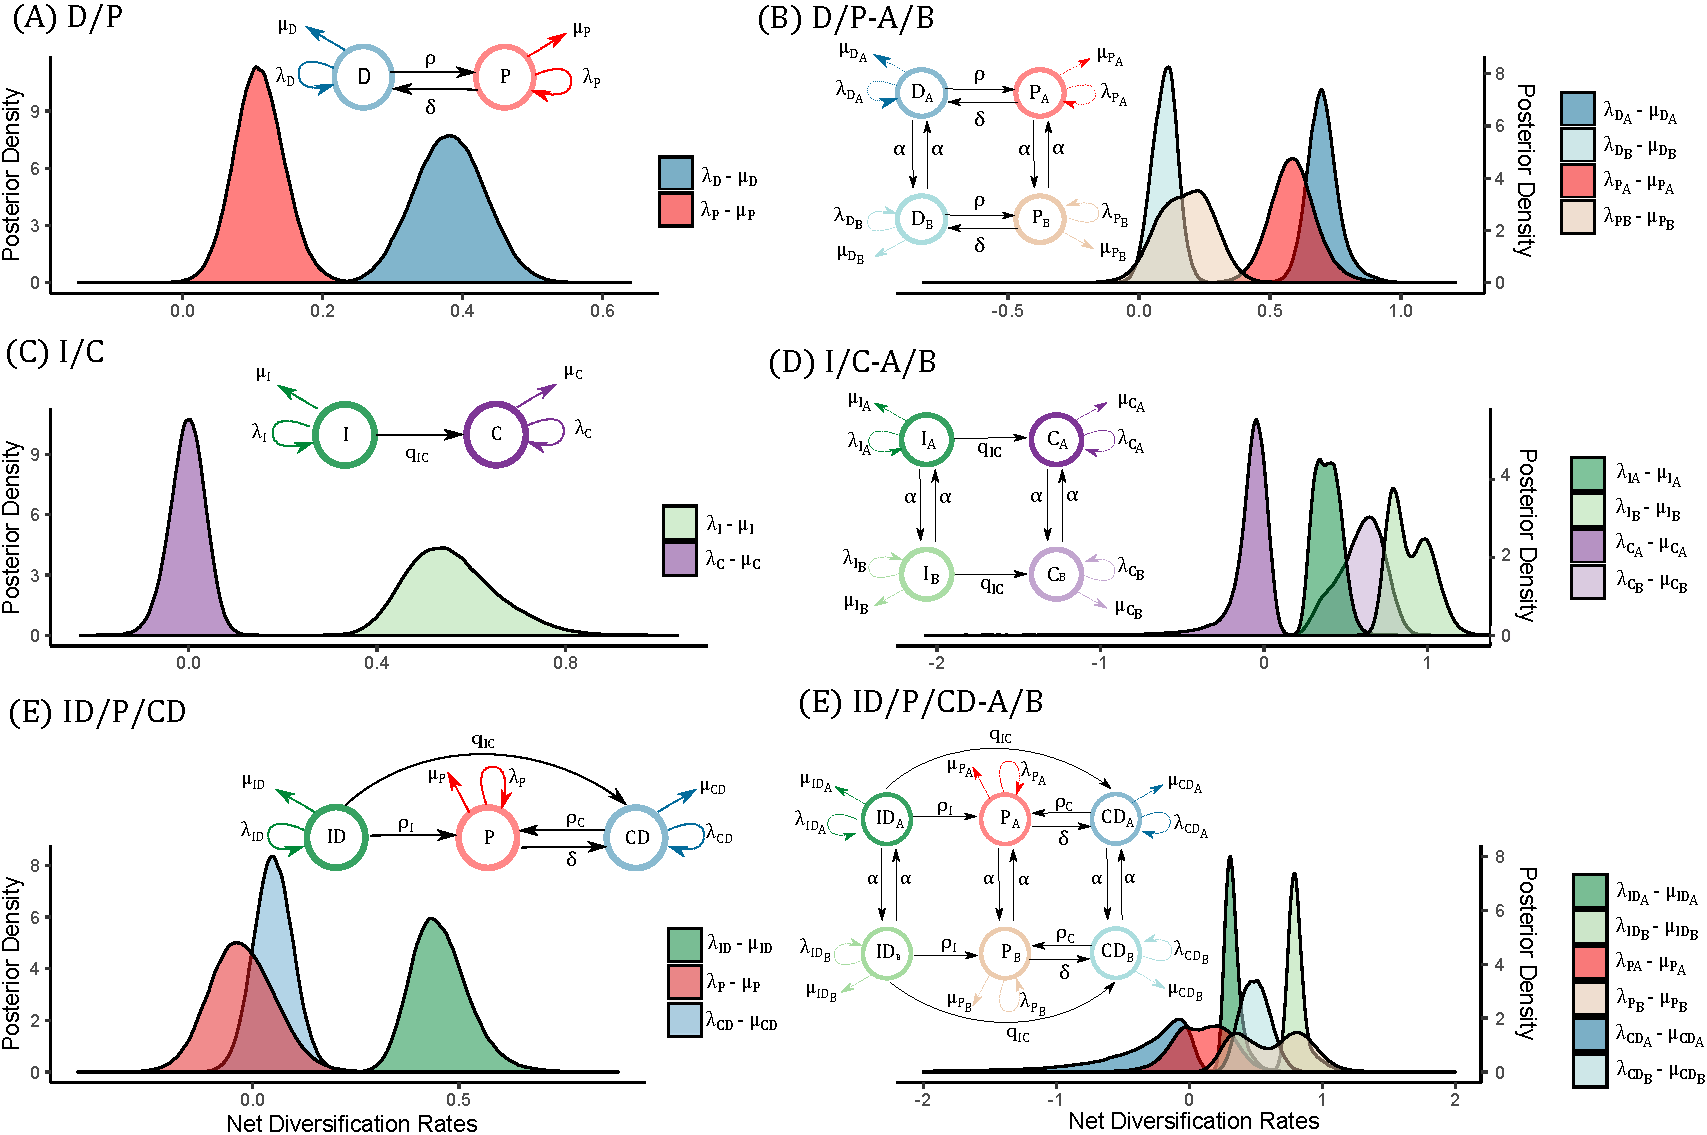
\includegraphics[width=\textwidth]{Netdiversificationallmodels.pdf}
  \caption{Net diversification rates for all models that include diploidization.}  
\label{figure:netdivall}
\end{figure}

\begin{figure}
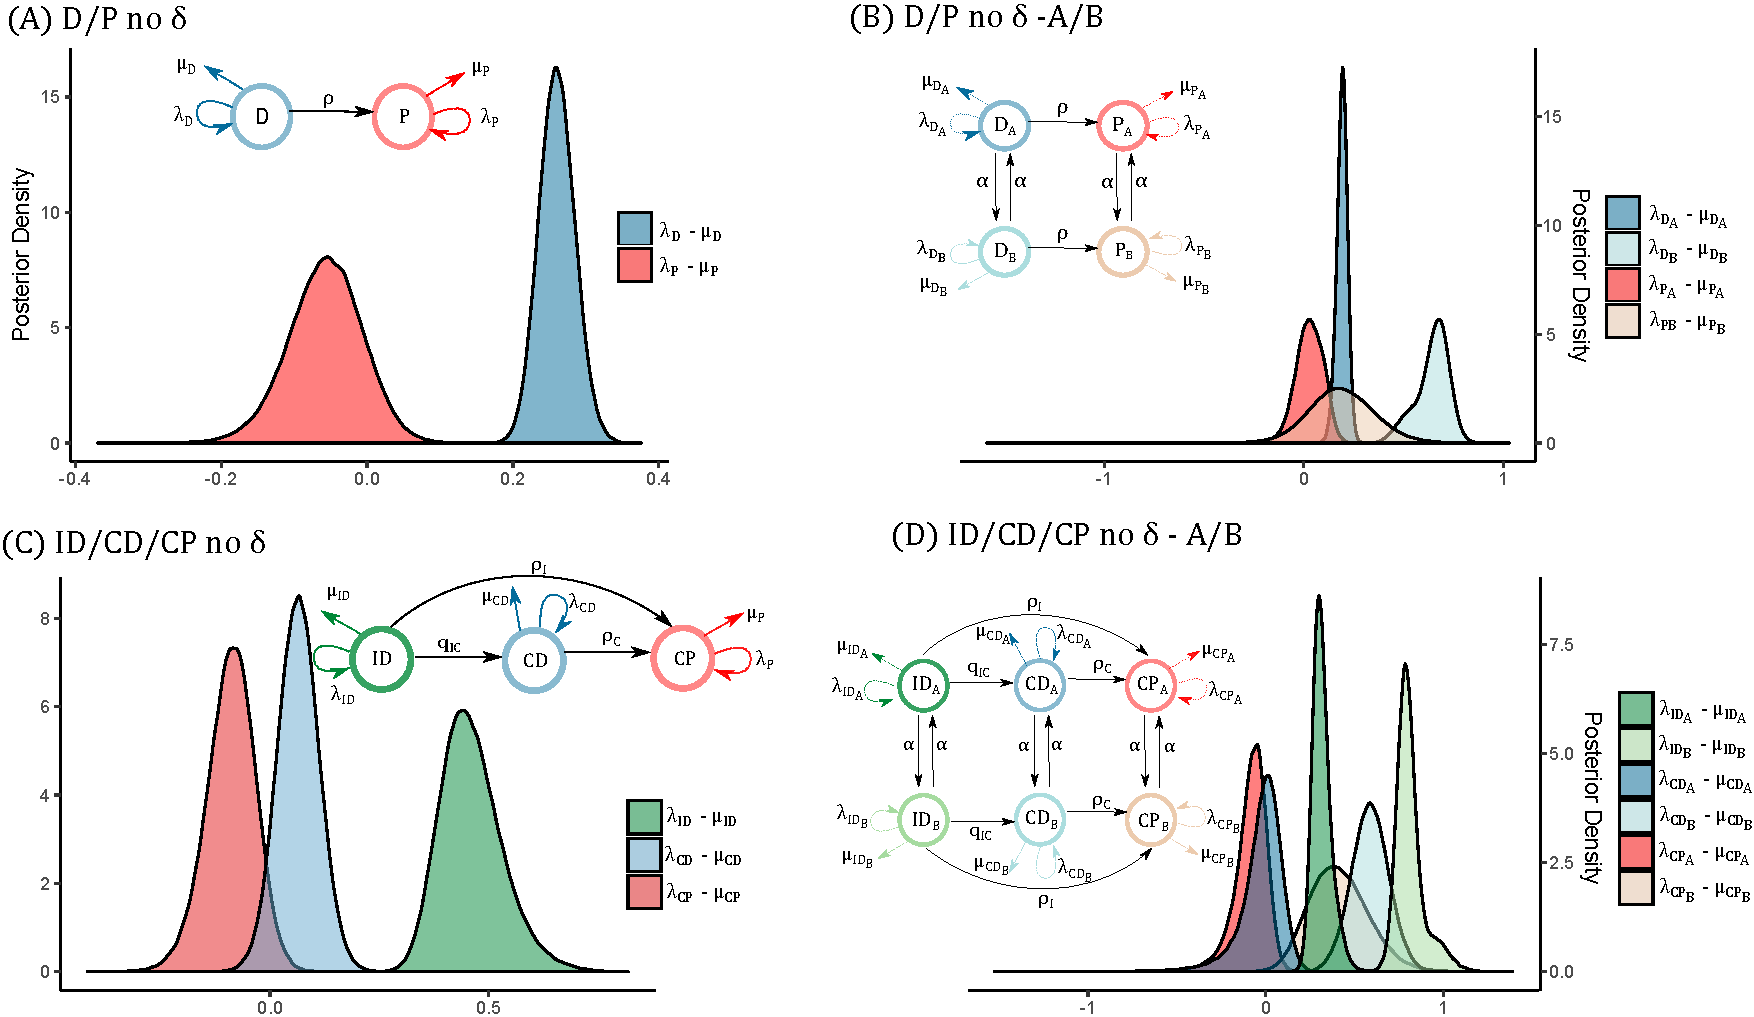
\includegraphics[width=\textwidth]{netdiversificationallnodip.pdf}
  \caption{Net diversification rates for all models that do not include diploidization.}  
\label{figure:netdivnodip}
\end{figure}

\begin{suppfigure}
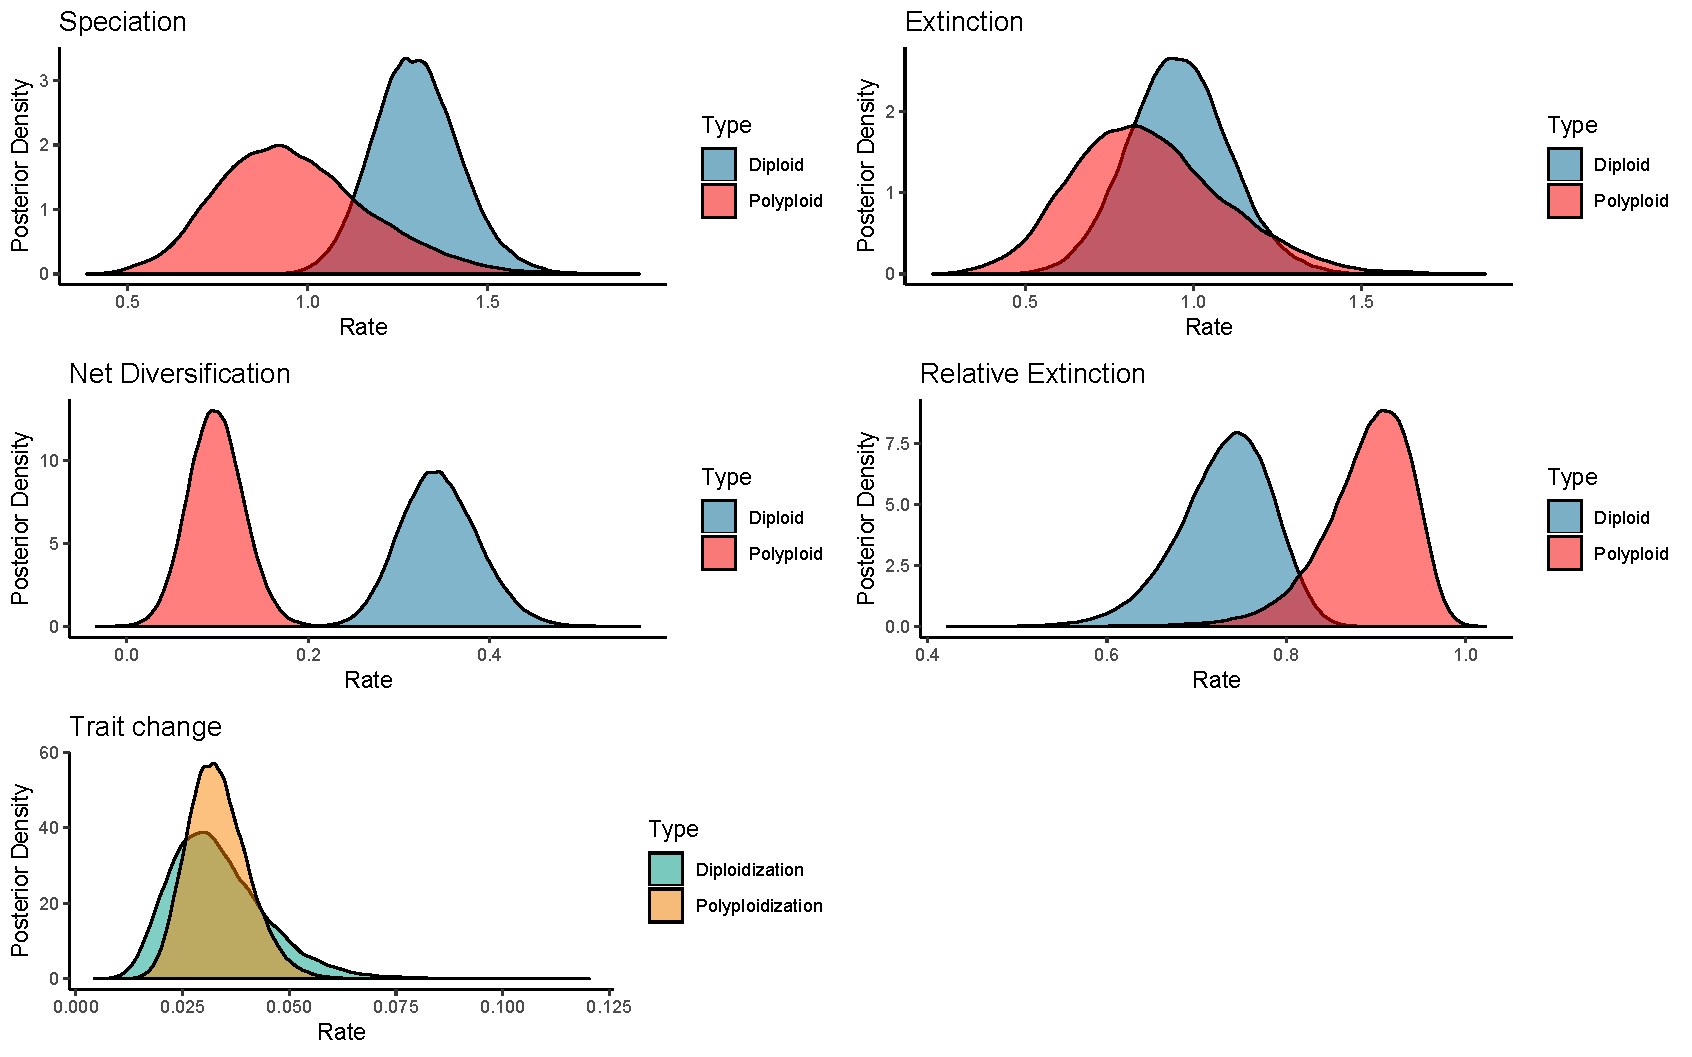
\includegraphics[width=\textwidth]{bisseDPposteriordist.pdf}
\caption{Posterior distribution for each of the parameters in the D/P polyploidy model} % XXX
\label{suppfigure:DP}
\end{suppfigure}

\begin{suppfigure}
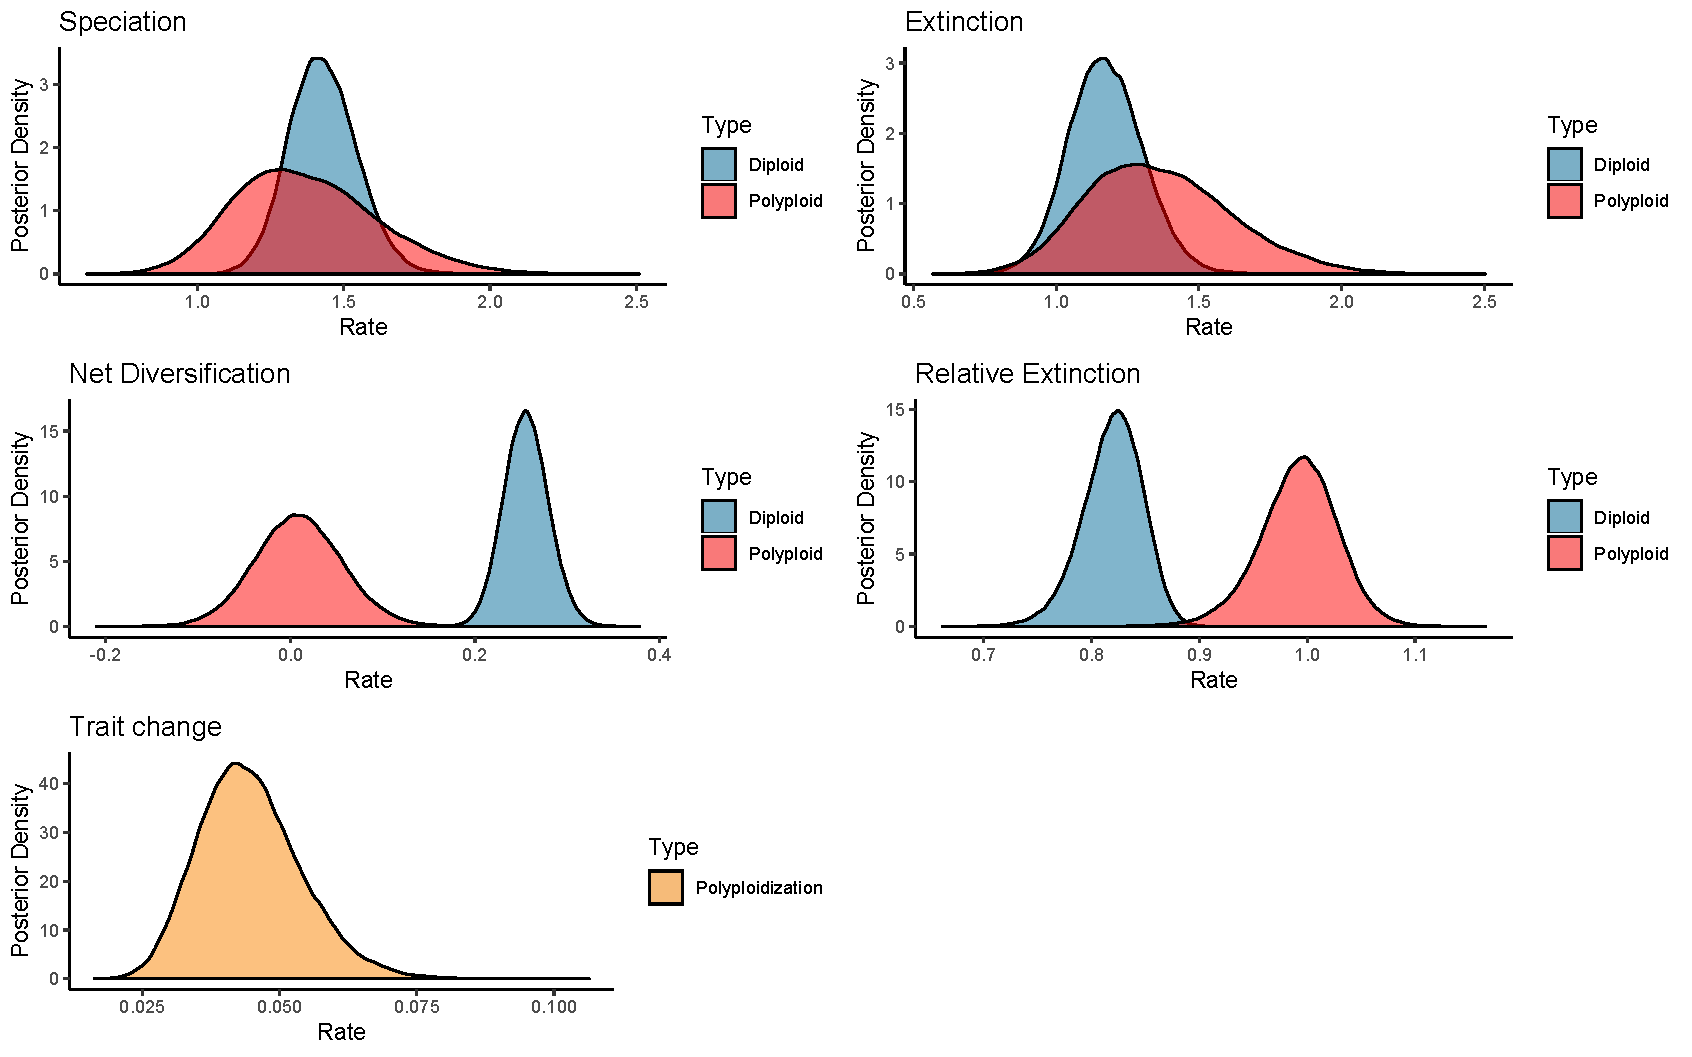
\includegraphics[width=\textwidth]{bisseDPnodipposteriordist.pdf}
\caption{Posterior distribution for each of the parameters in the D/P no $\delta$ polyploidy model} % XXX
\label{suppfigure:DPnodip}
\end{suppfigure}

\begin{suppfigure}
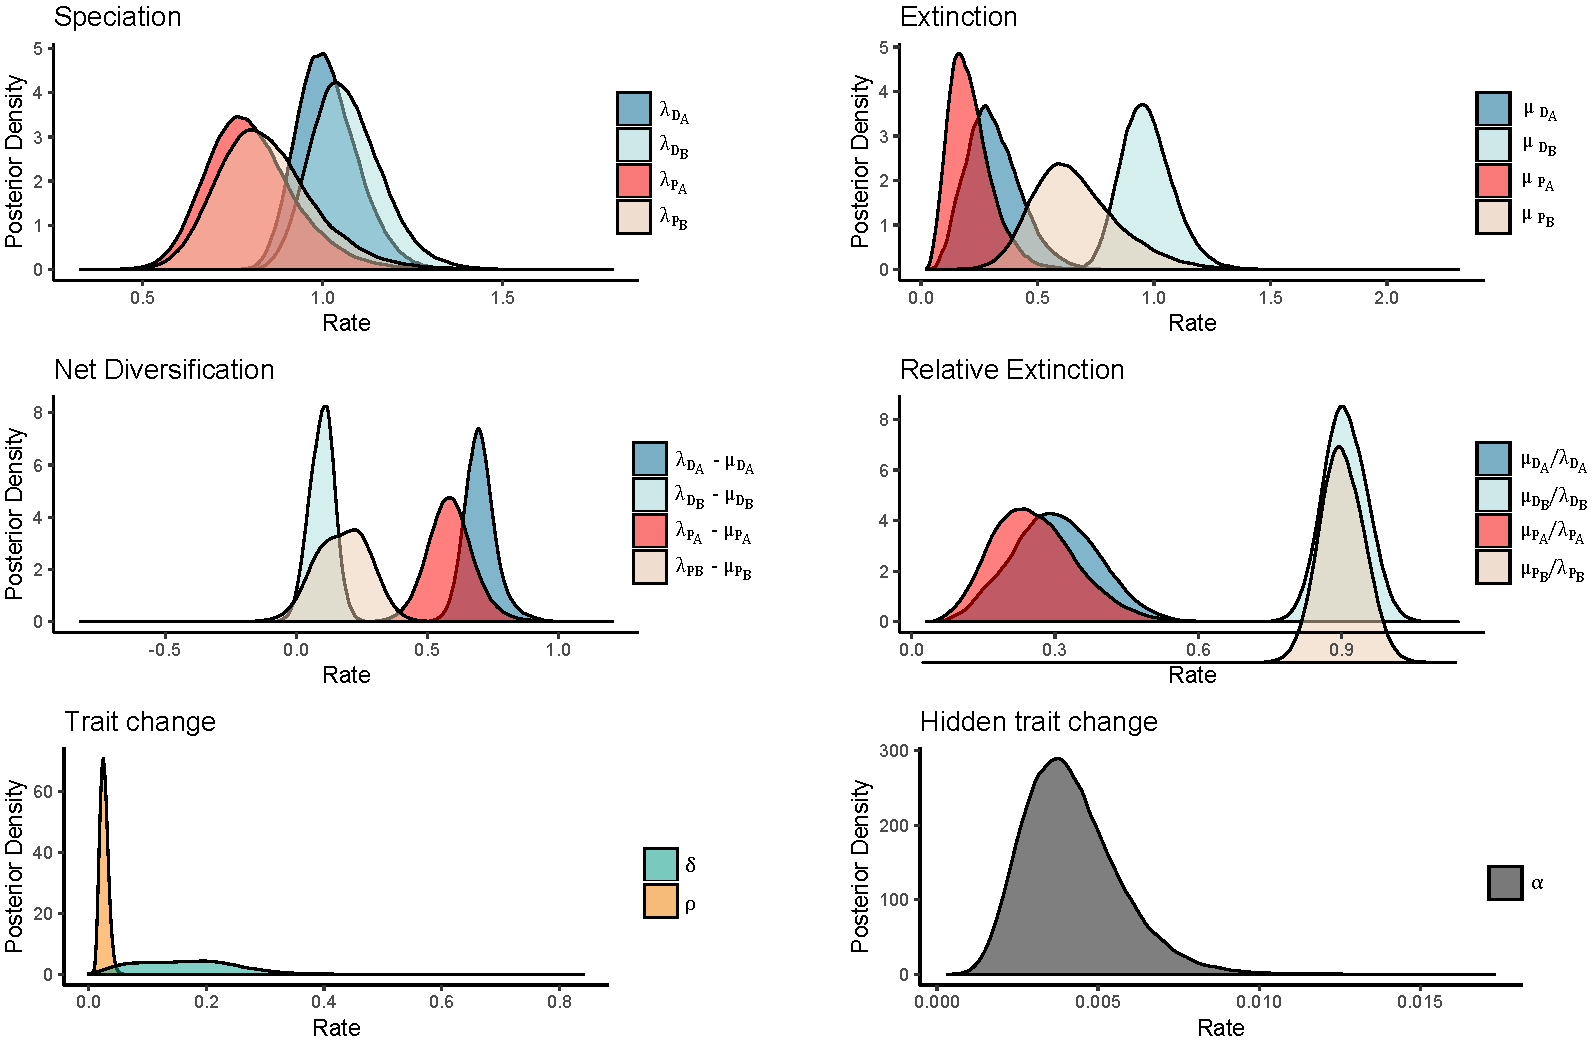
\includegraphics[width=\textwidth]{hisseDPposteriordist.pdf}
\caption{Posterior distribution for each of the parameters in the D/P-A/B polyploidy model} % XXX
% fixme: offset plotting error in "relative extinction" panel
\label{suppfigure:DPAB}
\end{suppfigure}

\begin{suppfigure}
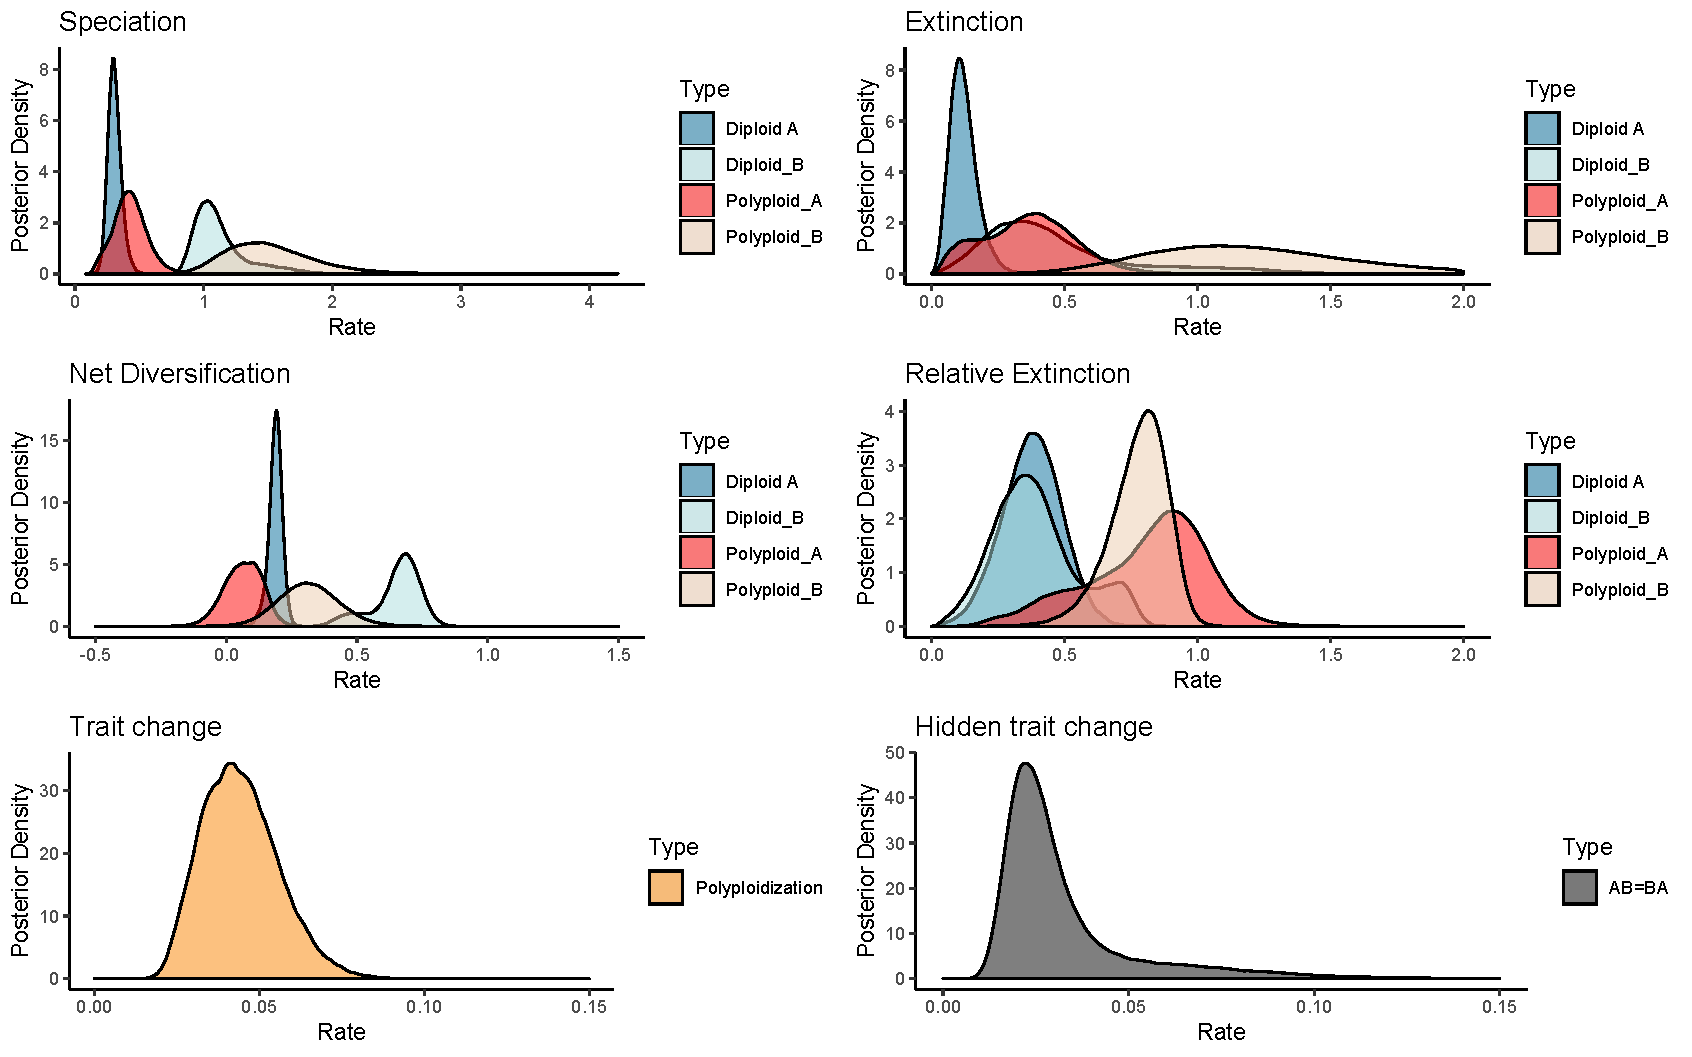
\includegraphics[width=\textwidth]{hisseDPnodipposteriordist.pdf}
\caption{Posterior distribution for each of the parameters in the D/P no $\delta$-A/B polyploidy model} % XXX
\label{suppfigure:DPnodipAB}
\end{suppfigure}

\begin{suppfigure}
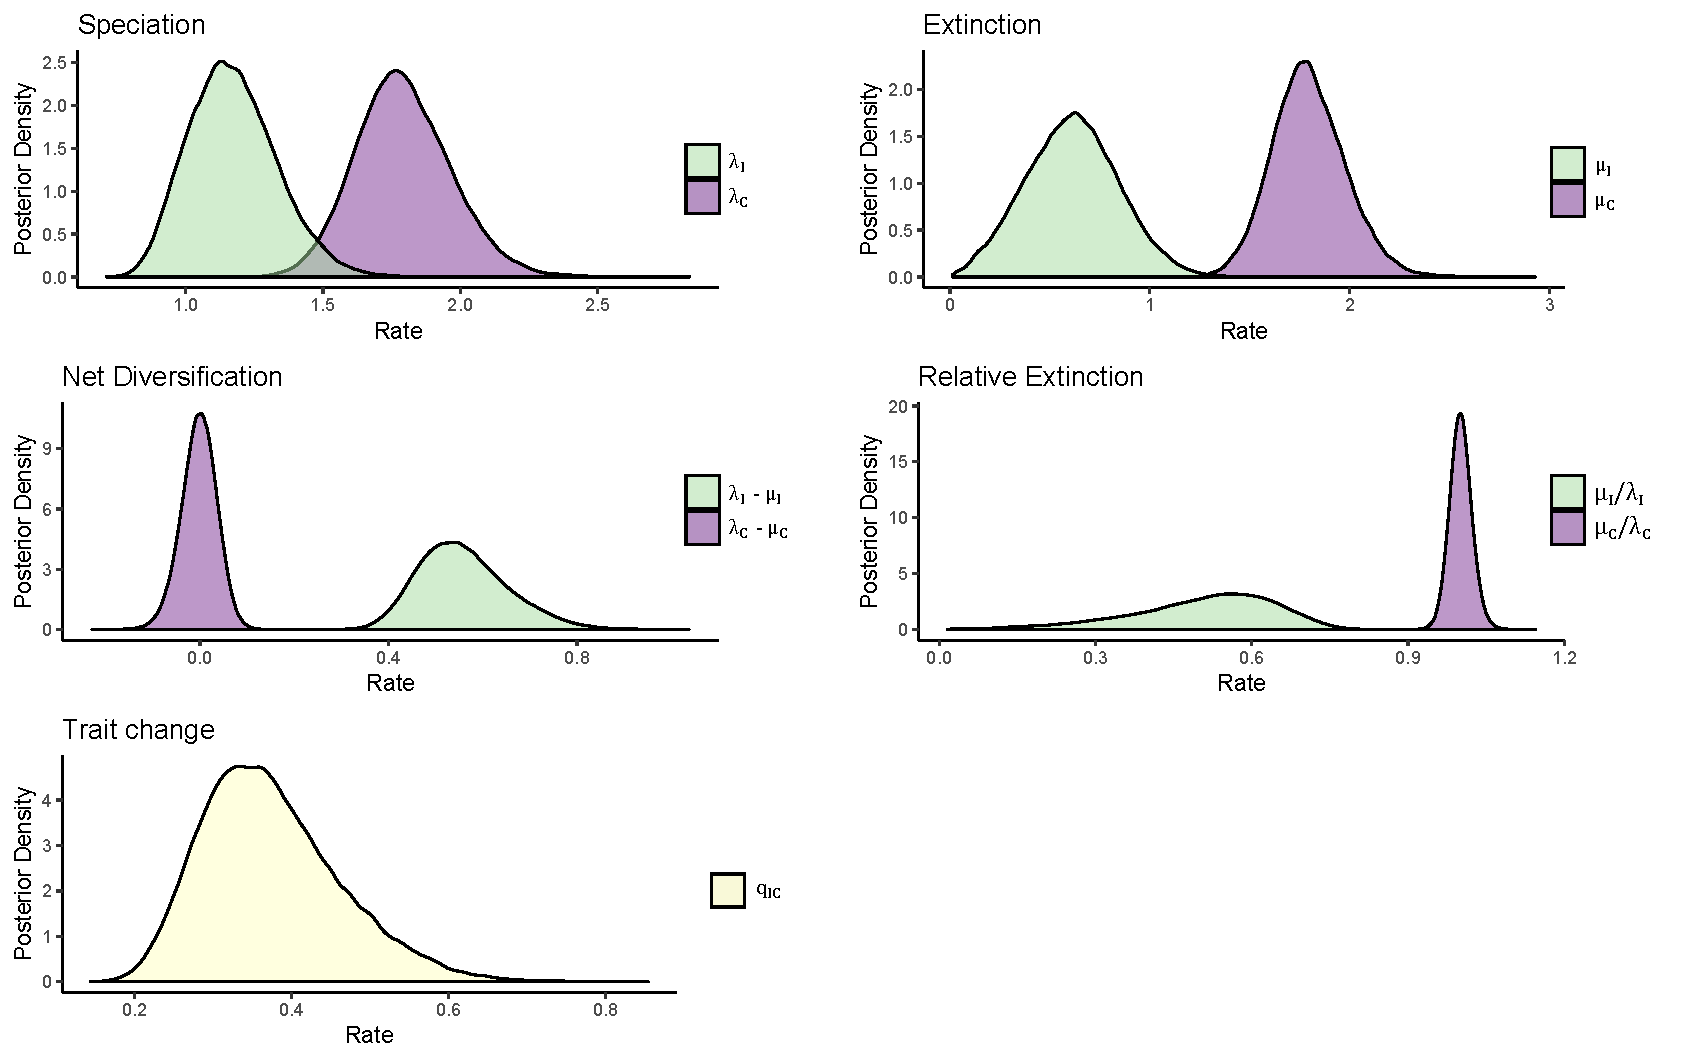
\includegraphics[width=\textwidth]{bisseSIposteriordist.pdf}
\caption{Posterior distribution for each of the parameters in the I/C breeding system model} % XXX
\label{suppfigure:IC}
\end{suppfigure}

\begin{suppfigure}
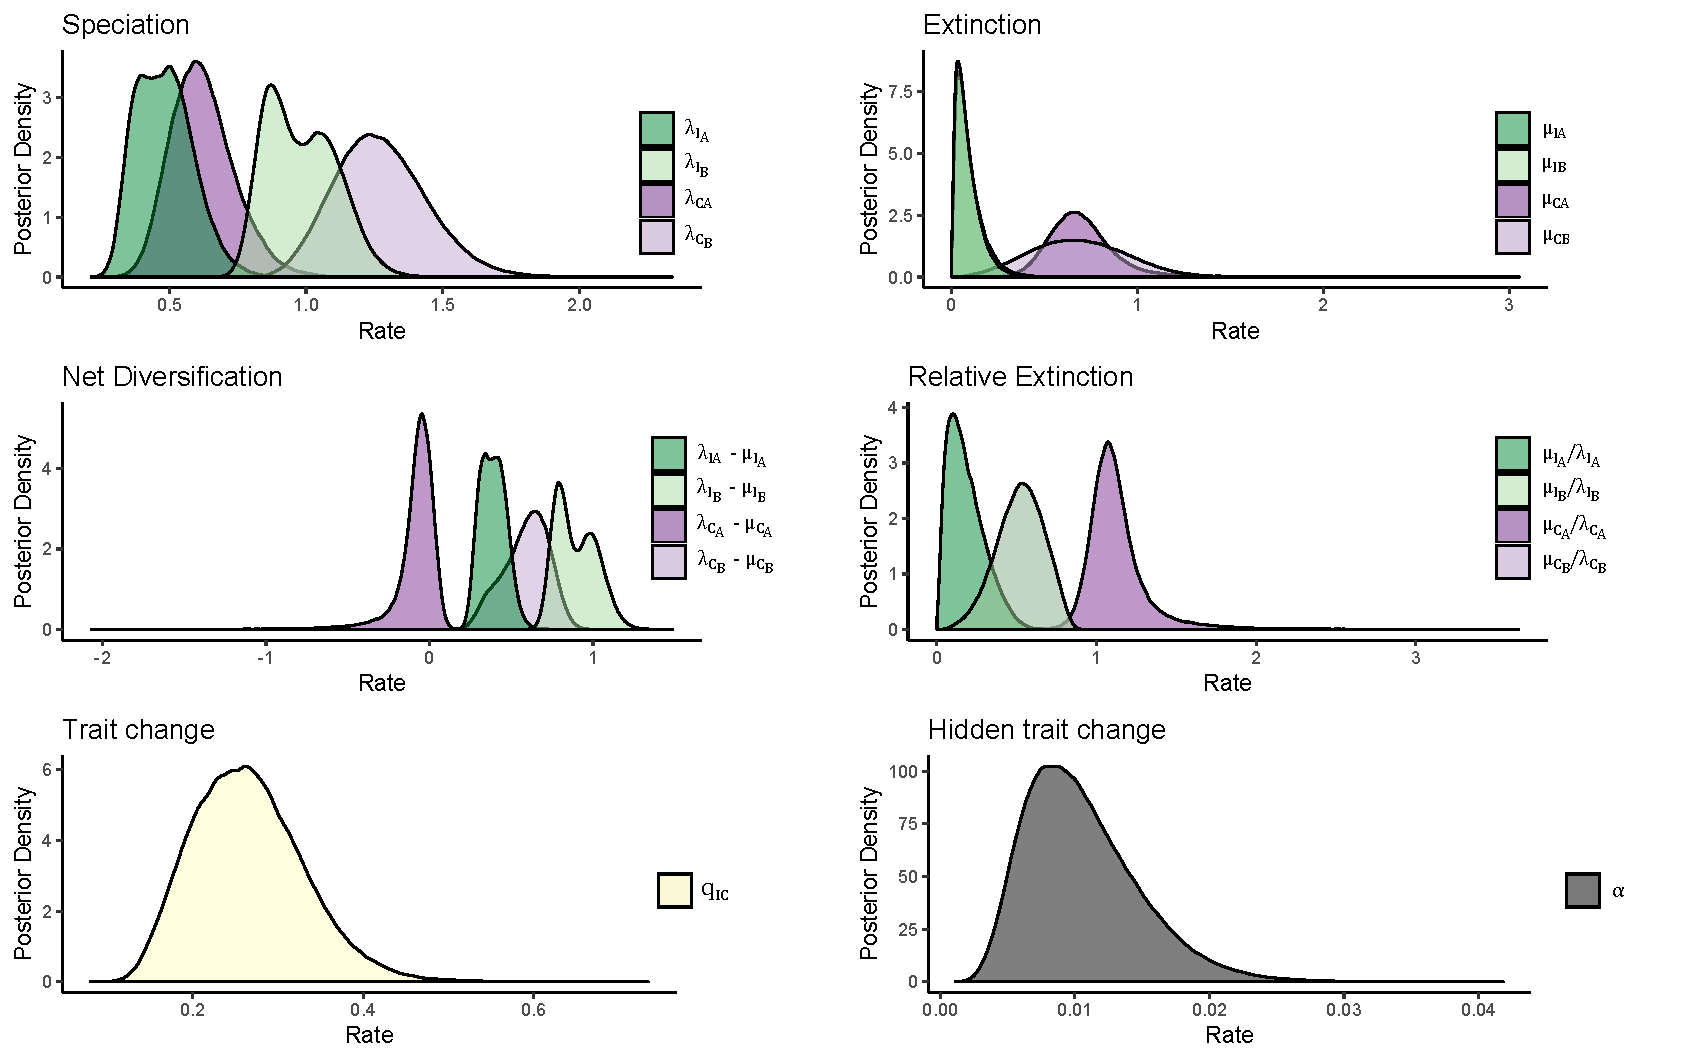
\includegraphics[width=\textwidth]{hisseSInoretposteriordist.pdf}
\caption{Posterior distribution for each of the parameters in the I/C-A/B breeding system model} % XXX
\label{suppfigure:ICAB}
\end{suppfigure}

\begin{suppfigure}
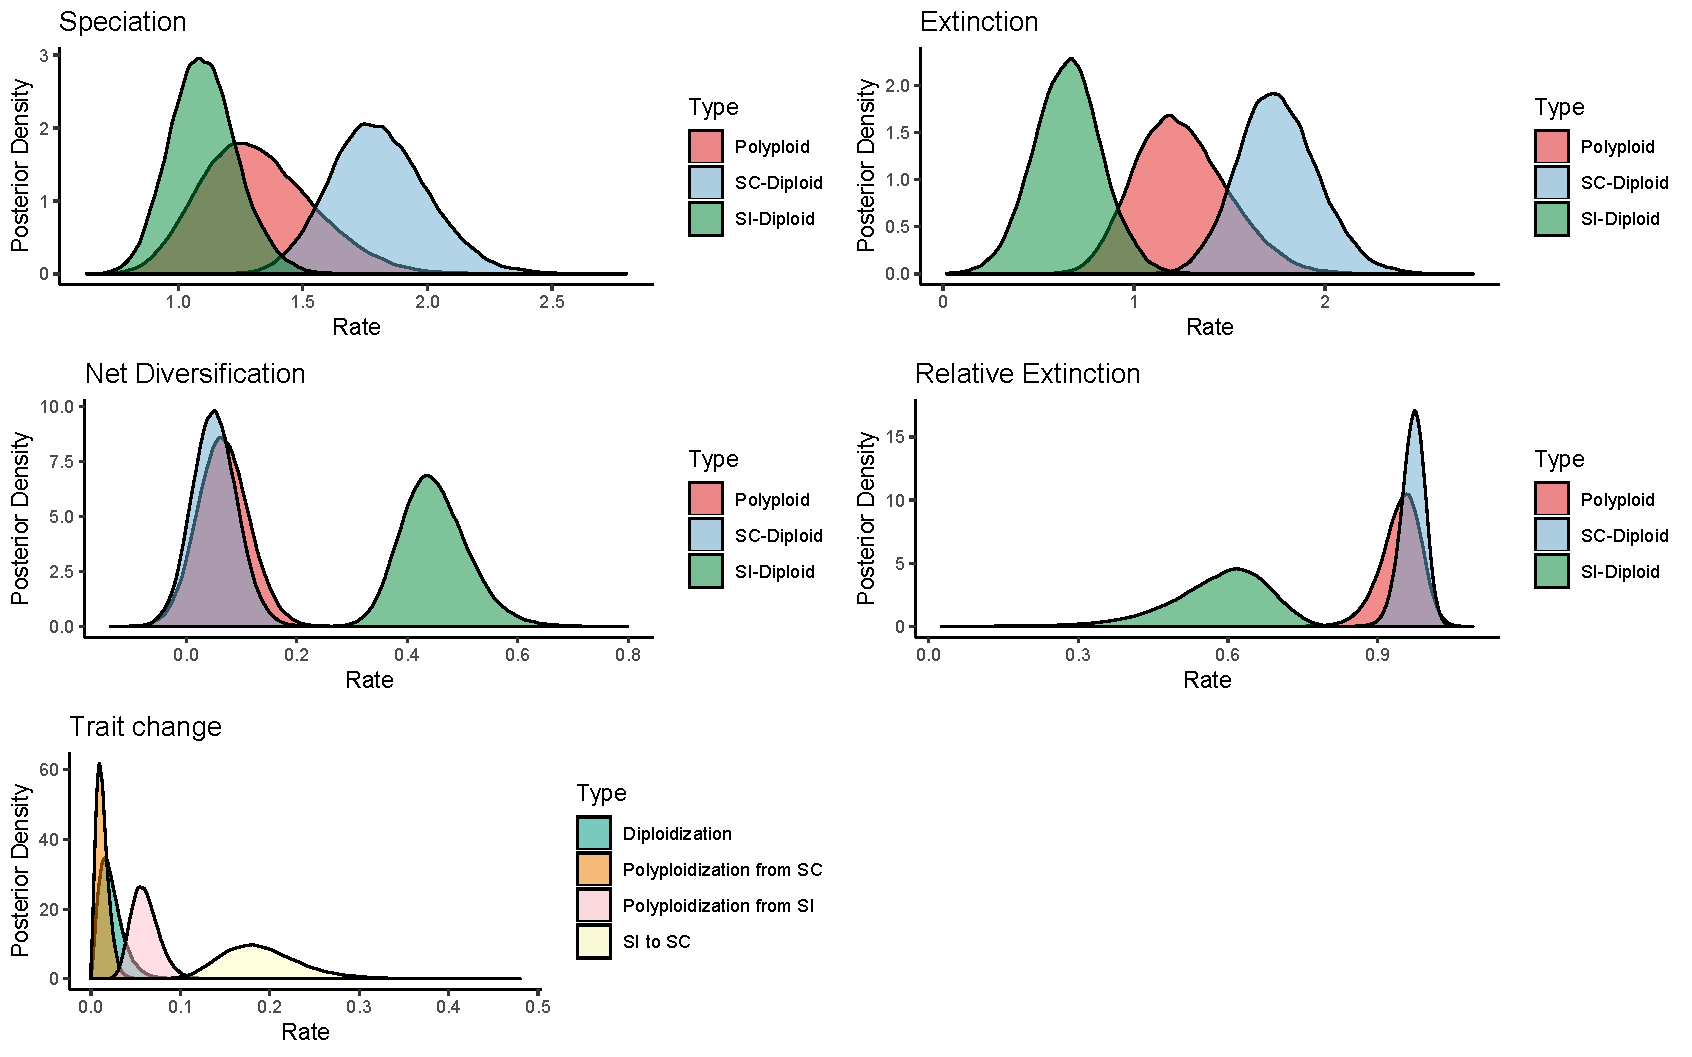
\includegraphics[width=\textwidth]{musseDPSIposteriordist.pdf}
\caption{Posterior distribution for each of the parameters in the ID/CD/CP polyploidy and breeding system model} % XXX
\label{suppfigure:IDCDCP}
\end{suppfigure}

\begin{suppfigure}
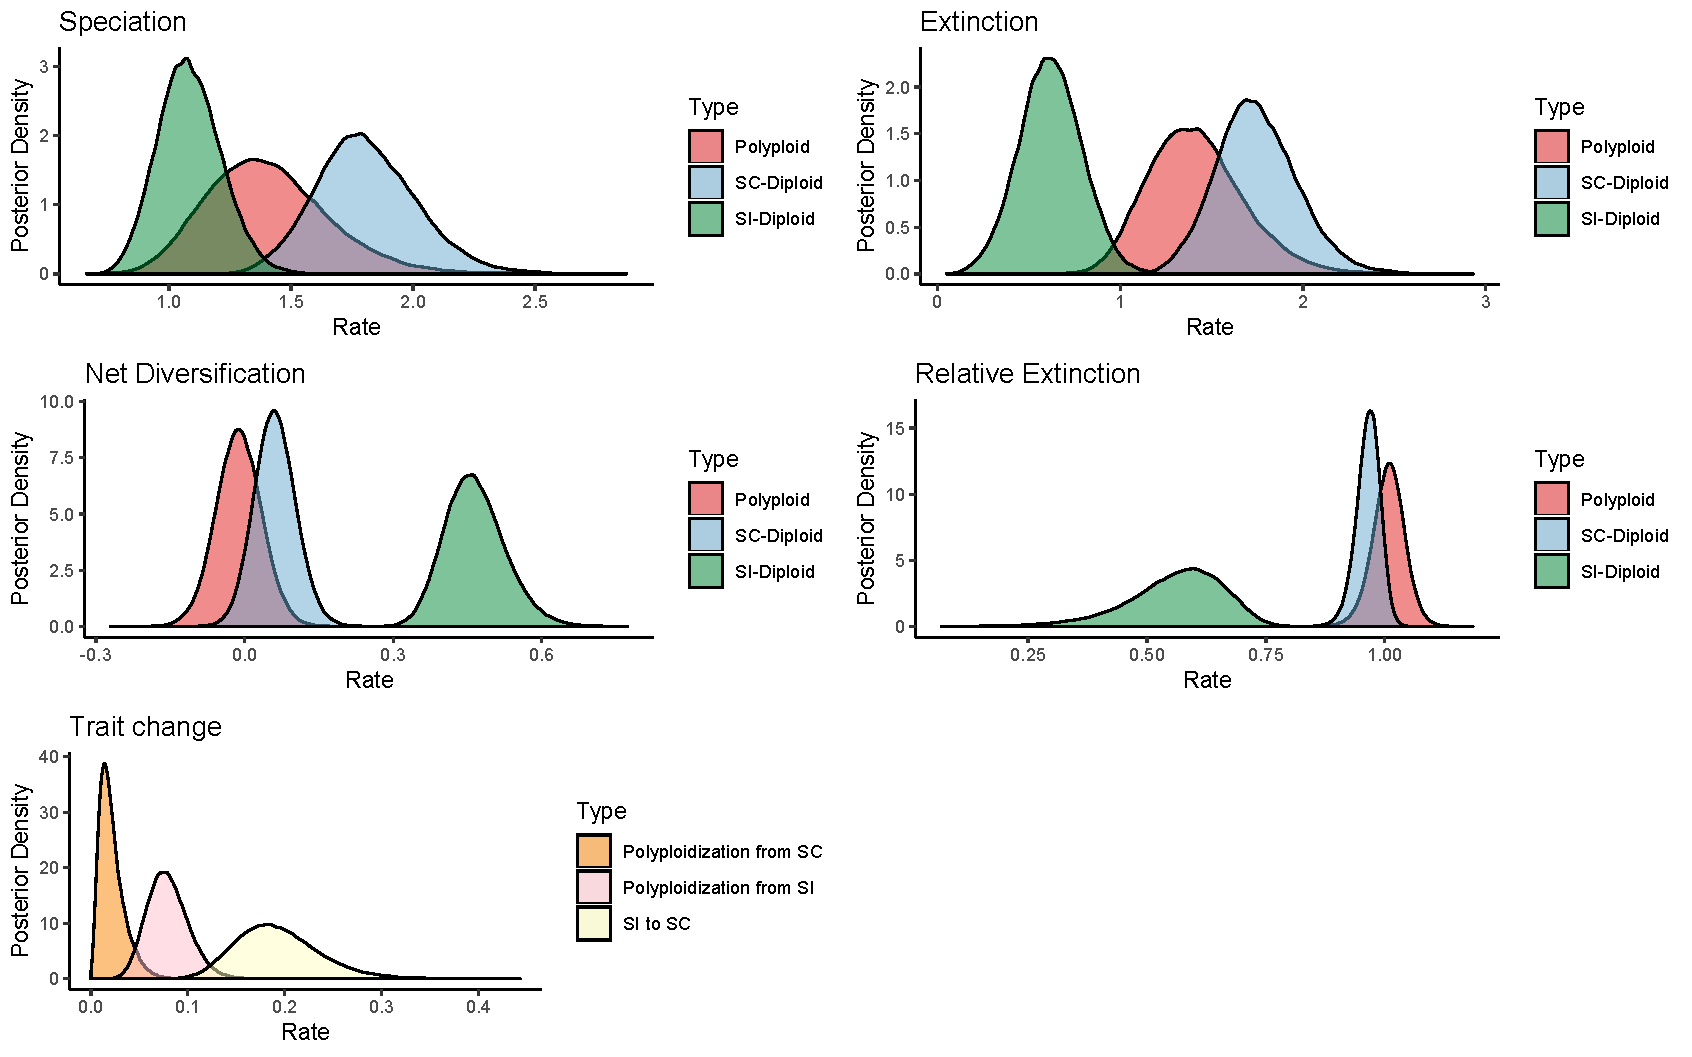
\includegraphics[width=\textwidth]{musseDPSInodipposteriordist.pdf}
\caption{Posterior distribution for each of the parameters in the ID/CD/CP no $\delta$ polyploidy and breeding system model} % XXX
\label{suppfigure:IDCDCPnodip}
\end{suppfigure}

\begin{suppfigure}
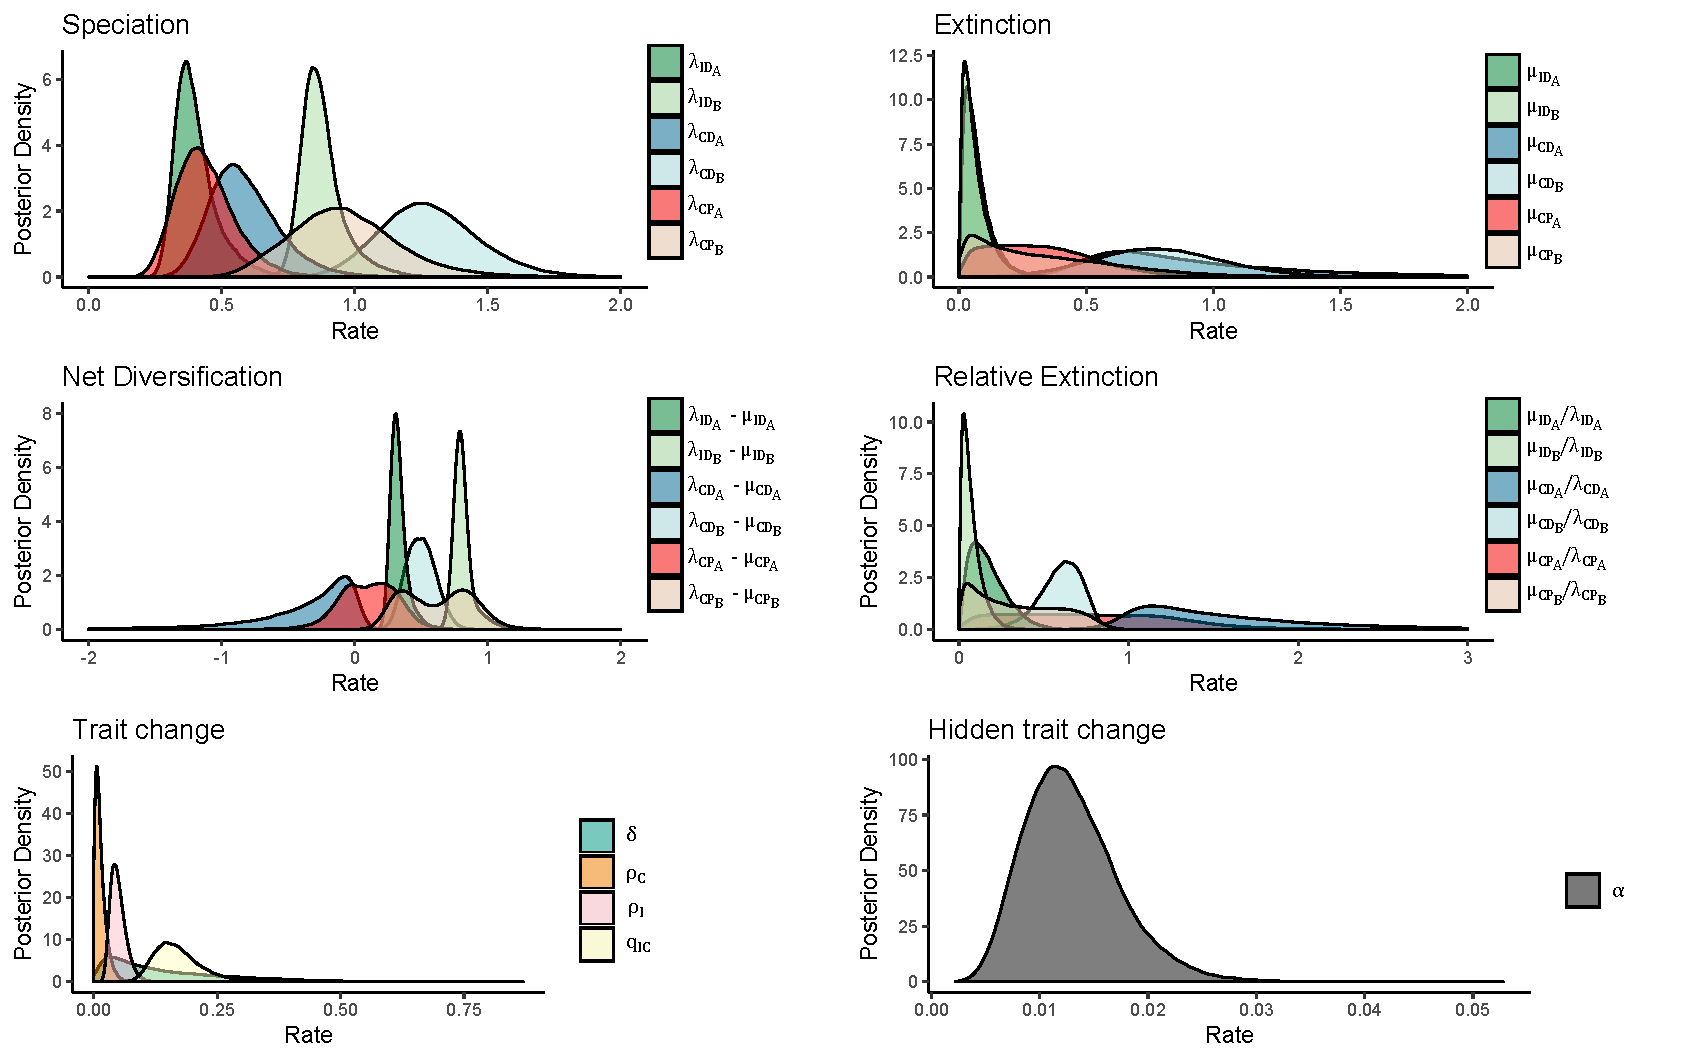
\includegraphics[width=\textwidth]{muhisseDPSIposteriordist.pdf}
\caption{Posterior distribution for each of the parameters in the ID/CD/CP-A/B polyploidy and breeding system model} % XXX
\label{suppfigure:IDCDCPAB}
\end{suppfigure}

\begin{suppfigure}
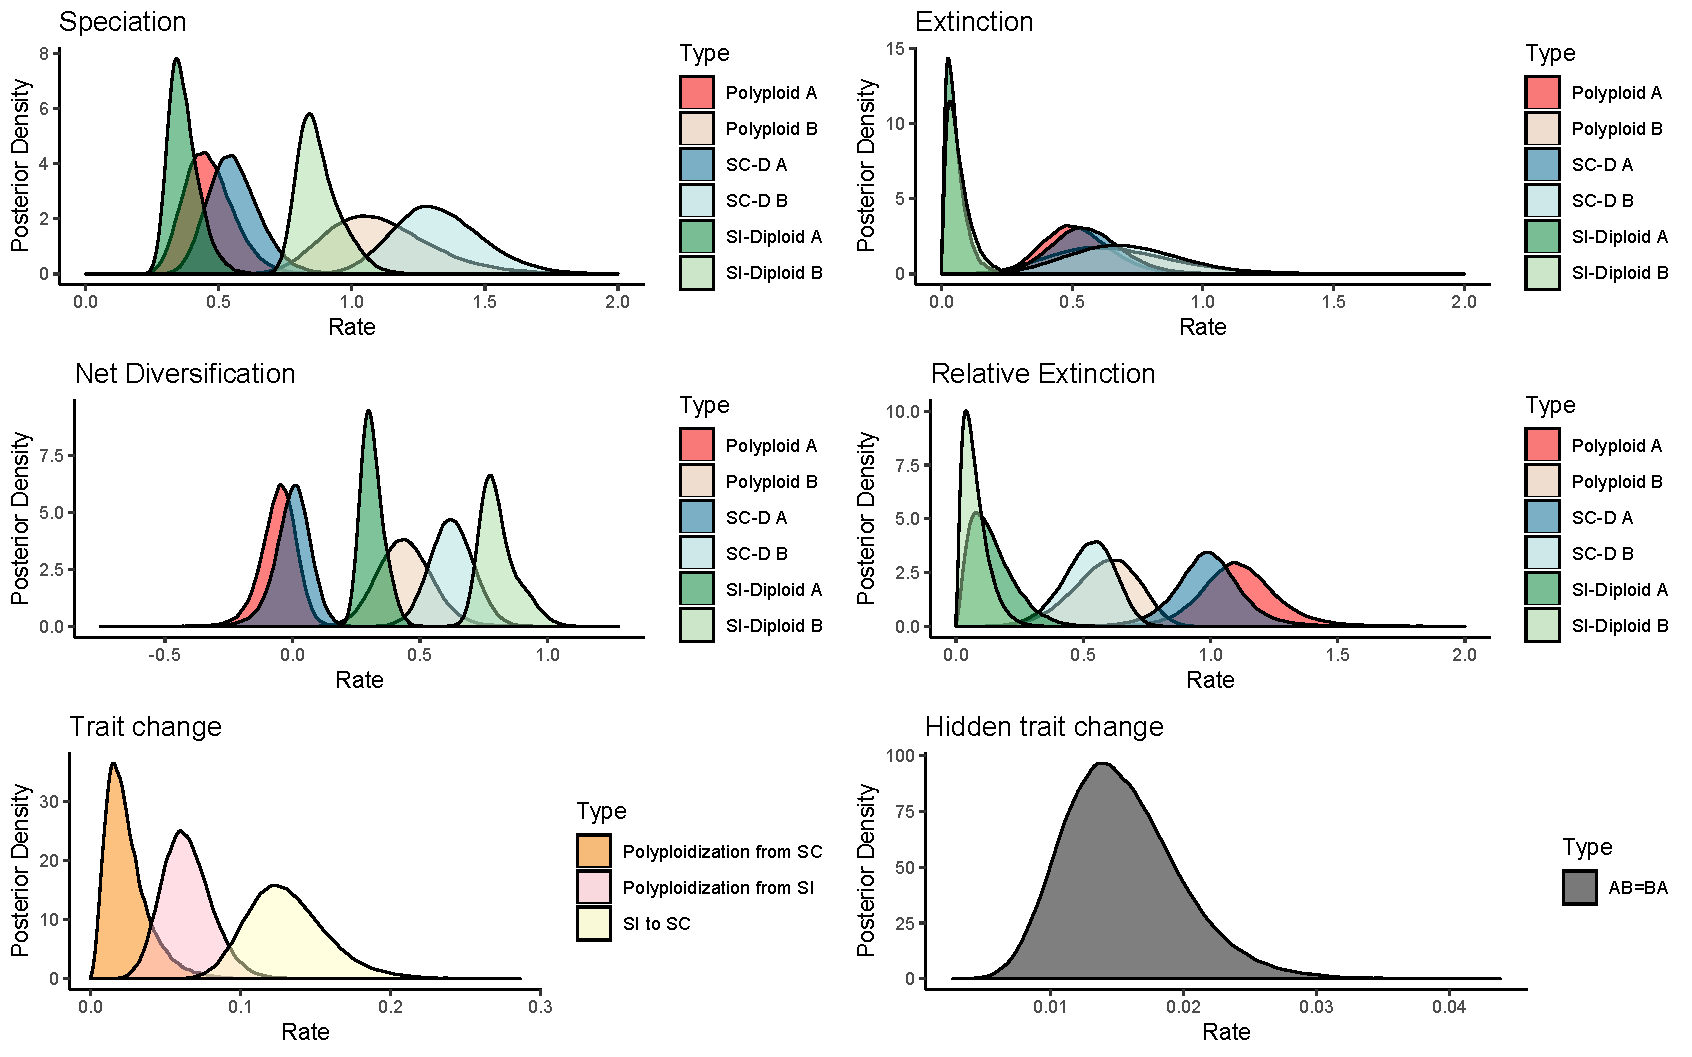
\includegraphics[width=\textwidth]{muhisseDPSInodipposteriordist.pdf}
\caption{Posterior distribution for each of the parameters in the ID/CD/CP no $\delta$- A/B polyploidy and breeding system model} % XXX
\label{suppfigure:IDCDCPnodipAB}
\end{suppfigure}

% E or R todo: which pathway from SI-D to SC-P is more common, based on rate estimates?  apply procedure from robertson2011 to rates from ID/CD/CP model
